\section{Experimental Setup and Results}
\label{sec:results}

\subsection{Data}
\label{sec:data}
No public benchmark with flood maps, delivery ground truth and georeferencing exists for the task of Section~\ref{sec:arch}. The evaluation therefore uses the three flood-annotated maps distributed with the \adapt{} repository (Table~\ref{tab:data}). They are \emph{demonstration inputs}, not a benchmark dataset. Two are news-style graphics in which detected flood pixels are drawn as red dots over a web-map basemap; the third is a thematic flood-hazard map with a legend. The PNG files contain no georeferencing: their only metadata are colour-profile chunks and a screen resolution of 5669~px/m. No manually annotated ground-truth masks exist, so segmentation accuracy (IoU, precision, recall) cannot be measured. The weather input is the repository's fixed weather file (Section~\ref{sec:weather}); the live API was only smoke-tested. Synthetic images with known geometry are used for geospatial verification (Section~\ref{sec:verres}).

\begin{table}[t]
\centering
\caption{Input data. All inputs are third-party demonstration images without georeferencing; ``source'' is the attribution printed on the image.}
\label{tab:data}
\footnotesize
\setlength{\tabcolsep}{2.5pt}
\begin{tabular}{@{}lllp{3.5cm}@{}}
\toprule
Map & Size (px) & Display & Content and printed source\\
\midrule
Varanasi & $972\times970$ & $750\times748$ & red flood dots on web basemap; ``ESA data \ldots processed by India Today''\\
Kanpur & $976\times966$ & $750\times742$ & red flood dots on web basemap; ``Sentinel-2 SAR data \ldots ESA'' (sic)\\
Assam & $1048\times739$ & $750\times529$ & thematic hazard map (5 classes, rivers, roads); no source printed\\
\bottomrule
\end{tabular}
\end{table}

\subsection{Setup and Protocol}
All experiments run the unmodified pipeline entry point on a laptop with an Intel Core i5-12500H CPU and 31.7~GiB RAM, under Windows~11 with Python~3.11.9, NumPy~2.4.6 and OpenCV~5.0.0, using the repository defaults (Table~\ref{tab:config}). Only three substitutions are made, all outside the pipeline code. Colour sampling is performed by a deterministic \emph{simulated operator} that clicks the centroids of the $K=8$ largest connected components of strongly saturated red pixels ($H\le5$ or $H\ge175$; $S,V>180$). Display windows are suppressed and their contents captured. The mission is written to the experiment folder instead of the default output path. All three maps use the repository's default geographic configuration, $(\varphi_0,\lambda_0)=(25.3176^\circ,82.9739^\circ)$ and $\rho=2.0$~m/px. All scripts, raw results and figure generators are provided with the paper (Data Availability).

\begin{table}[t]
\centering
\caption{Pipeline configuration used in all experiments (repository defaults).}
\label{tab:config}
\footnotesize
\setlength{\tabcolsep}{3pt}
\begin{tabular}{@{}ll@{}}
\toprule
Parameter & Value\\
\midrule
Display width $D$; min.\ area $a_{\min}$ & 750 px; 200 px$^2$\\
HSV patch; $\delta_H$, $\delta_{SV}$; element $B$ & $11\times11$; 20, 30; $5\times5$\\
Weather $(P,V,\theta)$ & 10 mm, 30 km/h, 270$^\circ$\\
Horizon $T$; spread coefficients & 2 h; 5 mm/px, 10 km/h/px\\
Grid factor; snap radius & 5; 10 cells\\
Reference $(\varphi_0,\lambda_0)$ & $25.3176^\circ$, $82.9739^\circ$\\
Scale $\rho$ & 2.0 m/px\\
Cruise / drop altitude; loiter & 100 / 10 m; 5 s\\
Servo channel; PWM & 9; 2000~$\mu$s\\
\bottomrule
\end{tabular}
\end{table}

\subsection{Metrics}
We report the \emph{flood-mask fraction} (share of display pixels in $M$) and the corresponding obstacle fraction for $O$; the number of regions, which equals the number of deliveries; planned legs and \emph{no-path legs}, the latter flown as straight segments; endpoints moved off obstacles and endpoints that could not be moved (\emph{unsnappable}); route points, mission items and runtime. For the ablation we use \emph{route exposure}, the fraction of route length lying over a given pixel set, sampled every 0.5~px. For route ordering we use the ratio of the nearest-neighbour tour length to the optimum, and for geospatial verification the deviations in degrees, metres and pixels against the oracle.

\subsection{End-to-End Results}
\label{sec:e2e}
Table~\ref{tab:e2e} and Fig.~\ref{fig:pipeline} summarise the end-to-end runs. All three runs complete and produce missions that pass the validator with no errors or warnings. Path planning accounts for more than 99\% of runtime; every other stage takes less than 0.1~s. Three findings qualify these outcomes.
\begin{enumerate}
\item \emph{No-path legs.} Half of the Varanasi legs (8 of 16) and 6 of 33 Kanpur legs have no path on the planning grid. The mission therefore flies straight segments across obstacles on these legs (red segments in Fig.~\ref{fig:pipeline}d). The independent A* baseline (Section~\ref{sec:baselines}) confirms that these endpoints are genuinely disconnected on the grid: after snapping, they lie in free pockets enclosed by the inflated flood mask.
\item \emph{Segmentation failure on the thematic map.} For Assam, the sampled patches include white background, $\ell_S$ falls to $0$ and achromatic pixels pass the red hue test (Section~\ref{sec:method}-B). Of the image, 83.1\% is labelled flood, the whole map becomes a single region, and both endpoints of the only (zero-length) leg remain inside obstacles. The resulting 10-item mission is structurally valid but meaningless.
\item \emph{Geography.} All missions lie within about 2~km of the default reference, irrespective of the map content (Section~\ref{sec:geovalid}).
\end{enumerate}

\begin{table}[t]
\centering
\caption{End-to-end results (default configuration, simulated operator, fixed weather).}
\label{tab:e2e}
\footnotesize
\setlength{\tabcolsep}{3pt}
\begin{tabular}{@{}lrrr@{}}
\toprule
 & Varanasi & Kanpur & Assam\\
\midrule
Flood-mask fraction $M$ (\%) & 8.10 & 15.08 & 83.10\\
Obstacle fraction $O$ (\%) & 15.81 & 29.06 & 92.24\\
Regions = deliveries & 16 & 33 & 1\\
Planned legs / no-path legs & 16 / 8 & 33 / 6 & 0 / 0\\
Endpoints snapped / unsnappable & 30 / 0 & 68 / 0 & 0 / 4\\
Route points & 297 & 1010 & 3\\
Mission items & 364 & 1145 & 10\\
Route length at configured scale (km) & 5.66 & 18.78 & 0.00\\
Validator errors / warnings & 0 / 0 & 0 / 0 & 0 / 0\\
Total runtime (s) & 13.4 & 35.7 & 0.03\\
Share of runtime in planning & 99.4\% & 99.6\% & --\\
\bottomrule
\end{tabular}
\end{table}

\begin{figure*}[t]
\centering
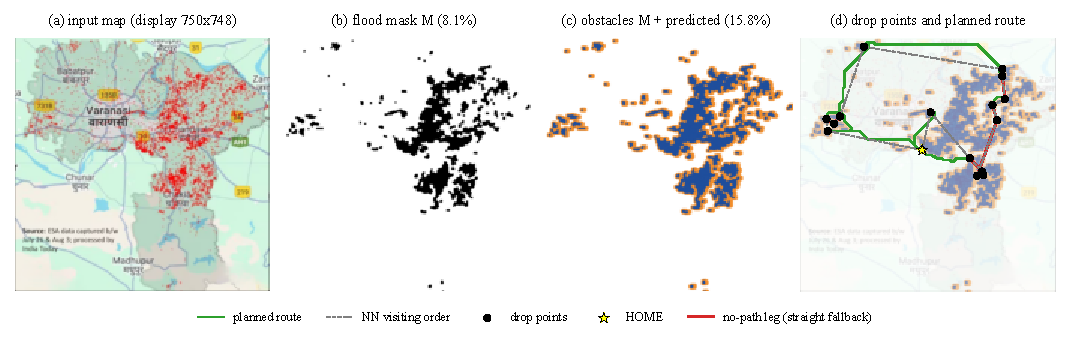
\includegraphics[width=0.92\textwidth]{figures/fig_pipeline.pdf}
\caption{Pipeline stages for the Varanasi map. (a) Input after display scaling (third-party map; see Data Availability). (b) Flood mask $M$. (c) Obstacles: $M$ (blue) and predicted-only pixels $\hat M\setminus M$ (orange). (d) Drop points, HOME, nearest-neighbour order (dashed), planned route (green) and the 8 no-path legs flown as straight segments (red).}
\label{fig:pipeline}
\end{figure*}

\subsection{Ablation: Predicted-Flood Obstacles}
Table~\ref{tab:ablation} and Fig.~\ref{fig:ablation} compare planning on $O=M\cup\hat M$ with planning on $M$ alone. Predicted-only pixels cover 7.7\% (Varanasi) and 14.0\% (Kanpur) of the image. Without predicted obstacles, 33.8\% and 47.9\% of the route length lies over predicted-only area. With them, exposure falls to 17.9\% and 11.6\%. Exposure does not reach zero because the no-path legs fly straight. The same inflation, however, causes \emph{all} no-path legs: there are none with $M$ alone, against 8 and 6 with $O$. It also increases planning time by a factor of 2.2--2.9, and for Varanasi it slightly increases exposure to the current flood (3.4\% to 4.8\%). The prediction stage is therefore not uniformly beneficial: in its current form, the benefit it is designed for comes with a loss of planner completeness.

\begin{table}[t]
\centering
\caption{Ablation of predicted-flood obstacles. Exposure is the share of route length over the given area.}
\label{tab:ablation}
\footnotesize
\setlength{\tabcolsep}{2.4pt}
\begin{tabular}{@{}llrrrrr@{}}
\toprule
Map & Obstacles & No-path & Items & Time (s) & \shortstack{Exposure\\pred.-only} & \shortstack{Exposure\\current}\\
\midrule
Varanasi & $M$ & 0 & 424 & 4.7 & 33.8\% & 3.4\%\\
 & $M\cup\hat M$ & 8 & 364 & 13.4 & 17.9\% & 4.8\%\\
Kanpur & $M$ & 0 & 733 & 16.5 & 47.9\% & 5.5\%\\
 & $M\cup\hat M$ & 6 & 1145 & 36.4 & 11.6\% & 4.3\%\\
\bottomrule
\end{tabular}
\end{table}

\begin{figure*}[t]
\centering
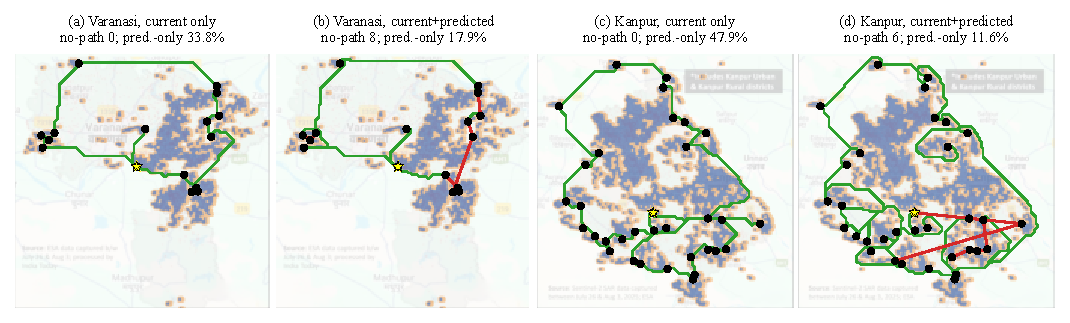
\includegraphics[width=0.92\textwidth]{figures/fig_ablation.pdf}
\caption{Planned routes with current-only obstacles (a, c) and with current and predicted obstacles (b, d). Blue: $M$; orange: $\hat M\setminus M$; red: no-path legs flown straight. Predicted obstacles move routes away from the predicted area but disconnect several drop points.}
\label{fig:ablation}
\end{figure*}

\subsection{Sensitivity}
Table~\ref{tab:sens} varies the colour margins and the number of operator clicks. The hue margin $\delta_H\in\{10,20,30\}$ has \emph{no} effect on any map, because the red-wrap rule replaces the hue interval. The saturation/value margin $\delta_{SV}\in\{15,30,45\}$ has a moderate effect on the two dot maps, while the Assam result is insensitive to every setting: its contamination is structural rather than a tuning artefact. Using 16 instead of 8 clicks raises the Varanasi flood fraction from 8.1\% to 9.7\% and the region count from 16 to 23, so the interactive step is a material source of variability. The ground scale $\rho$ affects only the geodetic conversion: the Varanasi route length scales linearly at 2.83~km per m/px, so the 5.66~km mission at $\rho=2$~m/px would be 263~km at the landmark-estimated scale of the map (Section~\ref{sec:geovalid}).

\begin{table}[t]
\centering
\caption{Sensitivity to the colour margin $\delta_{SV}$ and the number of clicks $K$ ($\delta_H=20$). Entries: flood-mask fraction (\%) / regions / no-path legs. Hue margins of 10, 20 and 30 give identical results.}
\label{tab:sens}
\footnotesize
\setlength{\tabcolsep}{3pt}
\begin{tabular}{@{}lccc@{}}
\toprule
Setting & Varanasi & Kanpur & Assam\\
\midrule
$\delta_{SV}=15$, $K=8$ & 7.2 / 19 / 8 & 14.0 / 32 / 6 & 83.1 / 1 / 0\\
$\delta_{SV}=30$, $K=8$ (default) & 8.1 / 16 / 8 & 15.1 / 33 / 6 & 83.1 / 1 / 0\\
$\delta_{SV}=45$, $K=8$ & 8.8 / 18 / 10 & 15.2 / 32 / 6 & 83.1 / 1 / 0\\
$\delta_{SV}=30$, $K=4$ & 8.1 / 16 / 8 & 15.1 / 33 / 6 & 83.1 / 1 / 0\\
$\delta_{SV}=30$, $K=16$ & 9.7 / 23 / 8 & 15.1 / 33 / 6 & 83.1 / 1 / 0\\
\bottomrule
\end{tabular}
\end{table}

\subsection{Route Ordering and Planner Baseline}
\label{sec:baselines}
Table~\ref{tab:baselines} reports two evaluation-only baselines; neither is part of \adapt{}. Against exact optima from Held--Karp dynamic programming \cite{held1962dynamic} on uniformly random instances, the nearest-neighbour order is on average 4.6\% (5 points) to 12.0\% (12 points) longer, with a worst case of 44.5\%. On the 16 Varanasi drop points it is 3.2\% longer than optimal. For the 33 Kanpur points only a minimum-spanning-tree lower bound is available, which limits the gap to at most 37.8\%.

The per-leg planner was compared with a plain grid A* \cite{hart1968formal} using the same grid, endpoints, costs and heuristic. The two agree on reachability for all 49 non-trivial legs and return equal path costs (difference below $2\times10^{-13}$), which supports the correctness of the D*~Lite implementation. As used in the pipeline, however, D*~Lite is 61 to 112 times slower than A*. Each leg builds a new instance and registers every obstacle cell, which amounts to 0.84 and 2.38 million vertex updates for the two maps, so its incremental design brings no benefit in this offline setting.

\begin{table}[t]
\centering
\caption{Evaluation-only baselines: route-ordering optimality and per-leg planner comparison.}
\label{tab:baselines}
\footnotesize
\setlength{\tabcolsep}{3pt}
\begin{tabular}{@{}lrrr@{}}
\toprule
\multicolumn{4}{@{}l}{\emph{Nearest neighbour / optimal tour length (random instances)}}\\
Points $n$ (instances) & Mean & Max & Optimal found\\
5 (300) & 1.046 & 1.257 & 42.3\%\\
8 (300) & 1.085 & 1.380 & 18.0\%\\
12 (100) & 1.120 & 1.445 & 11.0\%\\
Varanasi, $n=16$ & \multicolumn{3}{r}{1.032 (exact optimum)}\\
Kanpur, $n=33$ & \multicolumn{3}{r}{$\le$1.378 (MST bound)}\\
\midrule
\multicolumn{4}{@{}l}{\emph{Per-leg D*~Lite (as used) vs.\ grid A*, identical inputs}}\\
 & Varanasi & Kanpur & \\
Legs; reachability agreement & 16; 16/16 & 33; 33/33 & \\
Max.\ $|$cost difference$|$ & $4\times10^{-14}$ & $1\times10^{-13}$ & \\
Runtime D*~Lite / A* (s) & 12.67 / 0.21 & 30.83 / 0.28 & \\
\bottomrule
\end{tabular}
\end{table}

\subsection{Geospatial and Mission Verification}
\label{sec:verres}
Table~\ref{tab:verif} summarises the verification results; Fig.~\ref{fig:geodesy} shows resize consistency and model error. Every result in this subsection concerns \emph{software correctness}, that is, whether the code computes what its model specifies. None of it shows that the generated coordinates match real places.
\begin{itemize}
\item \emph{Synthetic ground truth.} On a $1000\times1000$~px synthetic image at 10~m/px, the implementation matches an independent re-derivation of \eqref{eq:enu}--\eqref{eq:geo} to within $1.4\times10^{-14}$~degrees at nine control points. Against the WGS84 geodesic ground truth, the largest error is 25.9~m at the image corners, dominated by the 0.49\% north--south scale error of $L$ at $25^\circ$, and every point is within the derived bound.
\item \emph{Round trips and edge cases.} Of 100\,000 randomised round trips through a test-only inverse, covering mid-latitudes, near-polar and near-antimeridian references, image sizes and scales from 0.05 to 633~m/px, 98\,789 are representable and agree within $6.8\times10^{-8}$~px; the remaining 1\,211 are correctly rejected.
\item \emph{Mission correspondence.} Every row of the three missions (1\,519 rows in total) matches an independent conversion of its source pixel within $3.6\times10^{-15}$~degrees. Traced back to the original image, the deviation is at most 0.57~m, entirely north--south and explained by the rounding of $H'$.
\item \emph{Resize consistency.} A synthetic three-region map run at nine display widths (300 to 2400~px, odd and even) yields drops at the same physical corners. They deviate from the model by at most one display pixel, and by $7\times10^{-10}$~m when no resizing occurs.
\item \emph{Mutation testing.} 22 of 24 injected defects are detected by the 126-test suite. The two surviving mutants are behaviour-equivalent: one removes a redundant finiteness guard, the other repeats a conversion.
\end{itemize}
During verification, the procedure exposed and led to the correction of defects in the original implementation: scale was not compensated after resizing, servo parameters were in the wrong slots, the region chosen as HOME received no delivery, the reference pixel was off by half a pixel, and invalid or polar inputs silently produced invalid coordinates. All results reported here use the corrected code.

\begin{table}[t]
\centering
\caption{Software verification of the geospatial and mission layers, and overall validation status.}
\label{tab:verif}
\footnotesize
\setlength{\tabcolsep}{3pt}
\begin{tabular}{@{}lr@{}}
\toprule
Check & Result\\
\midrule
\multicolumn{2}{@{}l}{\emph{Software correctness (performed)}}\\
Automated tests (incl.\ adversarial) & 126 + 494 subtests pass\\
Oracle vs.\ published geodesic & $\le$1 mm, $\le$0.01$''$\\
Implementation vs.\ model (synthetic) & $\le1.4\times10^{-14}$ deg\\
Model vs.\ WGS84, $\le$7.1 km offsets, 25$^\circ$ & $\le$25.9 m\\
Round trips (98\,789 compared) & max $6.8\times10^{-8}$ px\\
Mission rows vs.\ source pixels (1\,519) & $\le3.6\times10^{-15}$ deg\\
Resize, 9 display widths & $\le$1 display px\\
Mutants detected & 22/24 (2 equivalent)\\
Validator attack cases & 36 pass\\
Generated missions (3 maps) & 0 errors, 0 warnings\\
\midrule
\multicolumn{2}{@{}l}{\emph{Validation beyond software correctness}}\\
Geographic validity of supplied maps & not established\\
Ground-station load test (Mission Planner, QGC) & not performed\\
Software-in-the-loop (ArduPilot/PX4 SITL) & not performed\\
Hardware-in-the-loop / physical flight & not performed\\
\bottomrule
\end{tabular}
\end{table}

\begin{figure}[t]
\centering
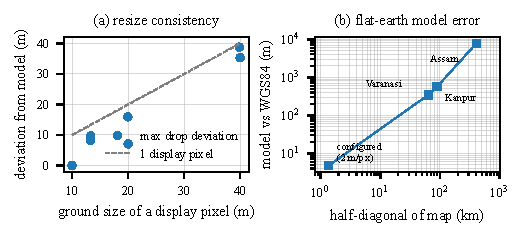
\includegraphics[width=\columnwidth]{figures/fig_geodesy.pdf}
\caption{(a) Maximum deviation of drop coordinates from the model across display widths, against the ground size of one display pixel. (b) Worst-case model error against WGS84 versus map half-diagonal: the configured 2~m/px setting and the landmark-estimated real extents of the three maps.}
\label{fig:geodesy}
\end{figure}

\subsection{Geographic Validity of the Supplied Maps}
\label{sec:geovalid}
To test whether the configured geography could describe the maps, a similarity transform was fitted between visible place-name labels and approximate public coordinates of those towns. This was done for 5, 10 and 12 labels on the Varanasi, Kanpur and Assam maps; the label positions were read off by eye. The estimate is a plausibility check, not a georeference. Residuals are 15--26~px and the rotations are $-0.5^\circ$, $-1.0^\circ$ and $-4.8^\circ$. The fitted scales are about 93, 130 and 633~m/px, which is 46, 65 and 317 times the configured 2.0~m/px. The default reference lies 23~km, 319~km and about 1\,000~km from the estimated image centres. At those extents, the flat-earth model itself would err by up to 345~m, 563~m and 7.7~km (Fig.~\ref{fig:geodesy}b), and the maps' web-Mercator basemaps violate the uniform-scale assumption \cite{battersby2014implications}. The generated missions are therefore \emph{not} geographically meaningful for these maps. The cause lies in the inputs and configuration, not in the conversion code.

\subsection{Mission Semantics}
The command parameters were audited against the MAVLink definitions and the ArduPilot and PX4 documentation \cite{mavlink_common,mavlink_mission,ardupilot_missioncmds,px4_missions}; the findings are given in Section~\ref{sec:method}-K and Section~\ref{sec:limits}. The lower block of Table~\ref{tab:verif} separates what has and has not been validated.
